\documentclass{article}

% packages
\usepackage{amsmath, amsthm, thmtools, amsfonts, amssymb, luacode, catchfile, tikzducks, hyperref, ifthen}
\ifcsname c@kobocompile\endcsname
	\usepackage[a5paper, total={1072pt, 1448pt}, margin=10pt, includeheadfoot]{geometry} % set page margins
\else
	\usepackage[a4paper, margin=50pt, includeheadfoot]{geometry}
\fi
\usepackage[shortlabels]{enumitem}
\usepackage[skip=3pt, indent=0pt]{parskip}

% language
\usepackage[bidi=basic, layout=tabular, provide=*]{babel}
\ifcsname c@english\endcsname
	\babelprovide[main, import]{english}
\else
	\babelprovide[main, import]{hebrew}
	\babelprovide{rl}
\fi
%\babelfont{rm}{Libertinus Serif}
\babelfont{rm}[Renderer=Harfbuzz]{Libertinus Serif}
\babelfont{sf}{Libertinus Sans}
\babelfont{tt}{Libertinus Mono}

% style
\AddToHook{cmd/section/before}{\clearpage}	% Add line break before section
\linespread{1.3}
\setcounter{secnumdepth}{0}		% Remove default number tags from sections, this won't do well with theorems
\AtBeginDocument{\setlength{\belowdisplayskip}{3pt}}
\AtBeginDocument{\setlength{\abovedisplayskip}{3pt}}
\graphicspath{ {../images/} }

% operators
\DeclareMathOperator\cis{cis}
\DeclareMathOperator\Sp{Sp}
\DeclareMathOperator\tr{tr}
\DeclareMathOperator\im{Im}
\DeclareMathOperator\re{Re}
\DeclareMathOperator\diag{diag}
\DeclareMathOperator*\lowlim{\underline{lim}}
\DeclareMathOperator*\uplim{\overline{lim}}
\DeclareMathOperator\rng{rng}
\DeclareMathOperator\Sym{Sym}
\DeclareMathOperator\Arg{Arg}
\DeclareMathOperator\Log{Log}
\DeclareMathOperator\dom{dom}
\DeclareMathOperator\supp{Supp}
\DeclareMathOperator\var{Var}
\DeclareMathOperator\cov{Cov}

% commands
%\renewcommand\qedsymbol{\textbf{מש''ל}}
%\renewcommand\qedsymbol{\fbox{\emoji{lizard}}}
\newcommand{\Aa}[0]{\mathcal{A}}
\newcommand{\Bb}[0]{\mathcal{B}}
\newcommand{\CC}[0]{\mathbb{C}}
\newcommand{\Cc}[0]{\mathcal{C}}
\newcommand{\EE}[0]{\mathbb{E}}
\newcommand{\FF}[0]{\mathbb{F}}
\newcommand{\Ff}[0]{\mathcal{F}}
\newcommand{\Ii}[0]{\mathcal{I}}
\newcommand{\Gg}[0]{\mathcal{G}}
\newcommand{\Ll}[0]{\mathcal{L}}
\newcommand{\Mm}[0]{\mathcal{M}}
\newcommand{\NN}[0]{\mathbb{N}}
\newcommand{\Nn}[0]{\mathcal{N}}
\newcommand{\PP}[0]{\mathbb{P}}
\newcommand{\Pp}[0]{\mathcal{P}}
\newcommand{\QQ}[0]{\mathbb{Q}}
\newcommand{\RR}[0]{\mathbb{R}}
\newcommand{\Rr}[0]{\mathcal{R}}
\newcommand{\Ss}[0]{\mathcal{S}}
\newcommand{\TT}[0]{\mathbb{T}}
\newcommand{\Uu}[0]{\mathcal{U}}
\newcommand{\Vv}[0]{\mathcal{V}}
\newcommand{\Ww}[0]{\mathcal{W}}
\newcommand{\ZZ}[0]{\mathbb{Z}}
\newcommand{\acts}[0]{\circlearrowright}
\newcommand{\explain}[2] {
	\begin{flalign*}
		 && \text{#2} && \text{#1}
	\end{flalign*}
}
\newcommand{\maketitleprint}[0]{ \begin{center}
	%\begin{tikzpicture}[scale=3]
	%	\duck[graduate=gray!20!black, tassel=red!70!black]
	%\end{tikzpicture}	
	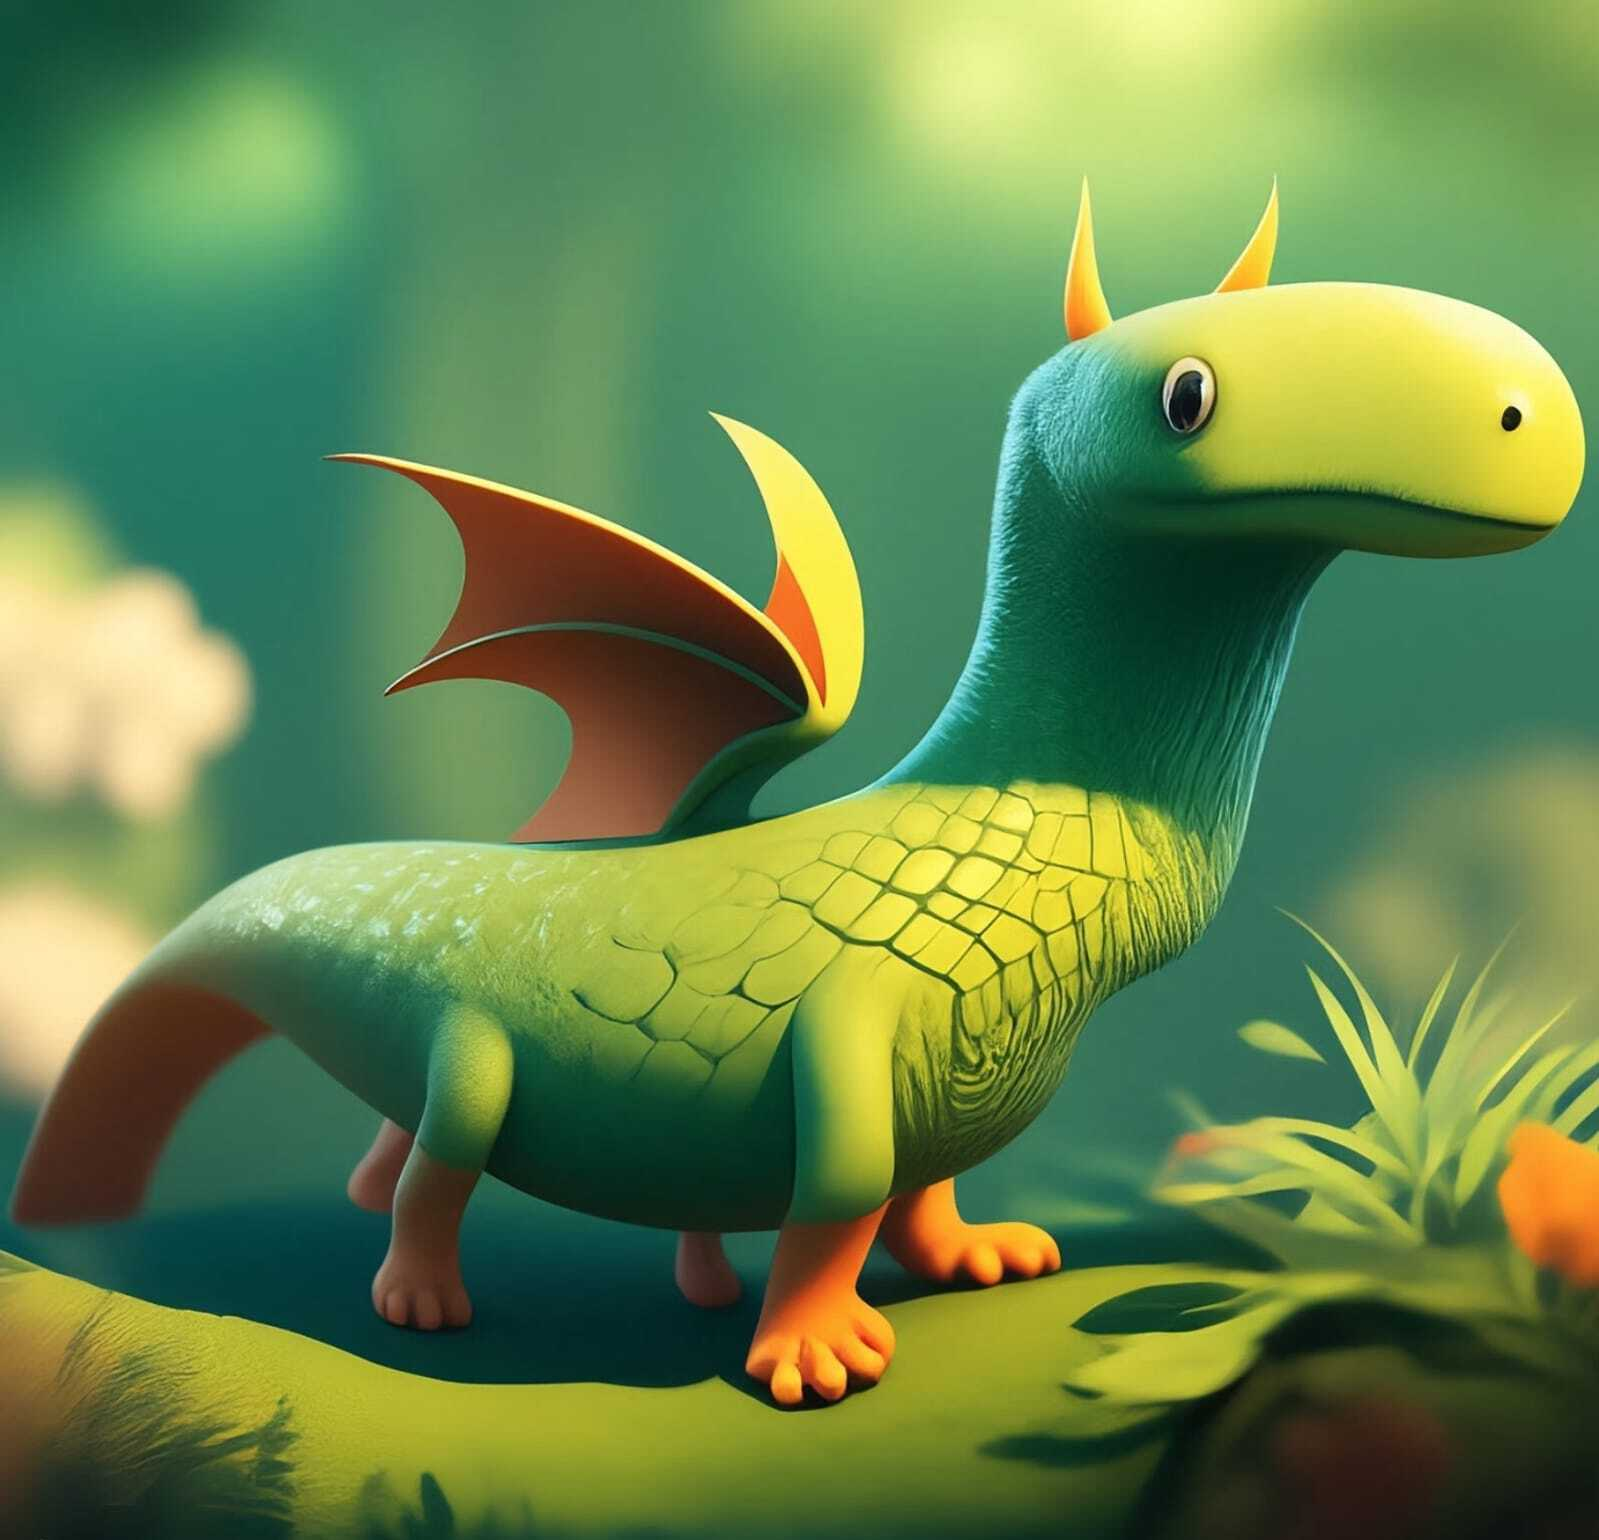
\includegraphics[width=6cm]{cover}
\end{center}
}

% theorem commands
\newtheoremstyle{c_remark}
	{}	% Space above
	{}	% Space below
	{}% Body font
	{}	% Indent amount
	{\bfseries}	% Theorem head font
	{}	% Punctuation after theorem head
	{.5em}	% Space after theorem head
	{\thmname{#1}\thmnumber{ #2}\thmnote{ \normalfont{\text{(#3)}}}}	% head content
\newtheoremstyle{c_definition}
	{3pt}	% Space above
	{3pt}	% Space below
	{}% Body font
	{}	% Indent amount
	{\bfseries}	% Theorem head font
	{}	% Punctuation after theorem head
	{.5em}	% Space after theorem head
	{\thmname{#1}\thmnumber{ #2}\thmnote{ \normalfont{\text{(#3)}}}}	% head content
\newtheoremstyle{c_plain}
	{3pt}	% Space above
	{3pt}	% Space below
	{\itshape}% Body font
	{}	% Indent amount
	{\bfseries}	% Theorem head font
	{}	% Punctuation after theorem head
	{.5em}	% Space after theorem head
	{\thmname{#1}\thmnumber{ #2}\thmnote{ \text{(#3)}}}	% head content

\ifcsname c@english\endcsname
	\theoremstyle{plain}
	\newtheorem{theorem}{Theorem}[section]
	\newtheorem{lemma}[theorem]{Lemma}
	\newtheorem{proposition}[theorem]{Proposition}
	\newtheorem*{proposition*}{Proposition}
	%\newtheorem{corollary}[theorem]{אין חלופה עברית}

	\theoremstyle{definition}
	\newtheorem{definition}[theorem]{Definition}
	\newtheorem*{definition*}{Definition}
	\newtheorem{example}{Example}[section]
	\newtheorem{exercise}{Exercise}[section]

	\theoremstyle{remark}
	\newtheorem*{remark}{Remark}
	\newtheorem*{solution}{Solution}
	\newtheorem{conclusion}[theorem]{Conclusion}
	\newtheorem{notation}[theorem]{Notation}
\else
	\theoremstyle{c_plain}
	\newtheorem{theorem}{משפט}[section]
	\newtheorem{lemma}[theorem]{למה}
	\newtheorem{proposition}[theorem]{טענה}
	\newtheorem*{proposition*}{טענה}
	%\newtheorem{corollary}[theorem]{אין חלופה עברית}

	\theoremstyle{c_definition}
	\newtheorem{definition}[theorem]{הגדרה}
	\newtheorem*{definition*}{הגדרה}
	\newtheorem{example}{דוגמה}[section]
	\newtheorem{exercise}{תרגיל}[section]

	\theoremstyle{c_remark}
	\newtheorem*{remark}{הערה}
	\newtheorem*{solution}{פתרון}
	\newtheorem{conclusion}[theorem]{מסקנה}
	\newtheorem{notation}[theorem]{סימון}
\fi

% Questions related commands
\newcounter{question}
\setcounter{question}{1}
\newcounter{sub_question}
\setcounter{sub_question}{1}

\ifcsname c@english\endcsname
	\newcommand{\question}[1][0]{
		\ifthenelse{#1 = 0}{}{\setcounter{question}{#1}}
		\section{Question \arabic{question}}
		\addtocounter{question}{1}
		\setcounter{sub_question}{1}
	}

	\newcommand{\subquestion}[1][0]{
		\ifthenelse{#1 = 0}{}{\setcounter{sub_question}{#1}}
		\subsection{Part \alph{sub_question}}
		\addtocounter{sub_question}{1}
	}
\else
	\newcommand{\question}[1][0]{
		\ifthenelse{#1 = 0}{}{\setcounter{question}{#1}}
		\section{שאלה \arabic{question}}
		\addtocounter{question}{1}
		\setcounter{sub_question}{1}
	}

	\newcommand{\subquestion}[1][0]{
		\ifthenelse{#1 = 0}{}{\setcounter{sub_question}{#1}}
		\subsection{סעיף \localecounter{letters.gershayim}{sub_question}}
		\addtocounter{sub_question}{1}
	}
\fi

% import lua and start of document
\directlua{common = require ('../common')}

\GetEnv{AUTHOR}

% headers
\author{\AUTHOR}
\date\today

\title{פתרון מטלה 01 --- מבנים אלגבריים (2), 80446}

\begin{document}
\maketitle
\maketitleprint{}

\question{}
תהי $L / K$ הרחבת שדות כך ש־$[L : K] = 7$.
נראה שלכל איבר $\alpha \in L \setminus K$ מתקיים $K[\alpha] = L$.
\begin{proof}
	נבחין כי מהגדרה $K[\alpha] \subseteq L$, וכן כמובן $K \subseteq K[\alpha]$.
	נוכל להניח גם ש־$K[\alpha]$ הוא שדה, זאת שכן $\alpha$ הפיך, ולכן מתקיים $[K : K[\alpha]] \cdot [K[\alpha] : L] = 7$.
	נבחין כי $[K : K[\alpha]] > 1$, אחרת $\alpha \in K$, ולכן מראשוניות נסיק ש־$[K[\alpha] : L] = 1$, כלומר $K[\alpha] = L$.
\end{proof}

\question{}
יהי $\FF$ שדה סופי,
נראה שיש $p$ ראשוני ו־$n \in \NN$ כך ש־$|\FF| = p^n$.
\begin{proof}
	נגדיר $p = \operatorname{char} \FF$, אילו $p = 0$ אז $|\FF| = \infty$ בסתירה, לכן נסיק ש־$p \in \NN$.
	נוכל אם כן להניח ש־$p$ ראשוני ומלמה מההרצאה נובע אף ש־$\FF_p \subseteq \FF$.
	אילו קיים ראשוני $q \mid |\FF|$, אז קיים איבר בשדה מהסדר הזה, לכן נסיק ש־$q = p$ בלבד, ולכן $|\FF| = p^n$ עבור איזשהו $n \in \NN$.
\end{proof}

\question{}
תהי $L / K$ הרחבת שדות ותהי $S = \{ s_i \mid 1 \le i \le m \} \subseteq L$.

\subquestion{}
נוכיח כי יש $K$־הומומורפיזם יחיד $\varphi : K[t_1, \dots, t_m] \to K[S]$ כך ש־$\varphi(t_i) = s_i$ לכל $i$.
\begin{proof}
	נניח כי $\varphi, \psi$ הומומורפיזמים המקיימים את הנתונים, אז $\forall i, \varphi(t_i) = \psi(t_i)$ מהגדרה.
	שתי ההעתקות סגורות לחיבור ולכפל, לכן אם $p_1, p_2 \in K[S]$ כך ש־$\varphi(p_j) = \psi(p_j)$ אז $\varphi(\alpha p_1 + \beta p_2) = \psi(\alpha p_1 + \beta p_2)$.
	לכן נותר שנבדוק הזדהות במונומים מתוקנים, כלומר איבר מהצורה $t_1^{\beta_1} \cdots t_m^{\beta_m}$,
	\[
		\varphi(t_1^{\beta_1} \cdots t_m^{\beta_m})
		= \varphi(t_1^{\beta_1}) \cdots \varphi(t_m^{\beta_m})
		= {\varphi(t_1)}^{\beta_1} \cdots {\varphi(t_m)}^{\beta_m}
		= {\psi(t_1)}^{\beta_1} \cdots {\psi(t_m)}^{\beta_m}
		= \psi(t_1^{\beta_1} \cdots t_m^{\beta_m})
	\]
	וקיבלנו כי אכן שתי ההעתקות מזדהות על כל התחום, כלומר $\varphi = \psi$.
\end{proof}

\subquestion{}
נפריך את הטענה כי יש $K$־הומומורפיזם יחיד $\varphi : K(t_1, \dots, t_m) \to K(S)$ כך ש־$\varphi(t_i) = s_i$ לכל $i$.
\begin{solution}
	נבחן את $\varphi : \RR(x) \to K(\{ i \}) = \CC$ עבור $K = \RR, L = \CC$.
	נניח שקיים $\varphi$ כזה, אז מתקיים $\varphi(x) = i$, ובהתאם נוכל להסיק בדומה לסעיף הקודם ש־$\varphi(f) = f(i)$ לכל פונקציה רציונלית $f \in \RR(x)$.
	לבסוף נובע $\varphi(\frac{1}{x^2 + 1}) = \frac{1}{i^2 + 1} = \frac{1}{0}$, כלומר הפונקציה לא מוגדרת היטב, וזו סתירה להנחת הקיום שלה.
\end{solution}

\question{}
יהי $\FF$ שדה ויהי $f \in \FF[x]$ פולינום מעל השדה.

\subquestion{}
נוכיח שאם $\deg f = 1$ אז $f$ ראשוני.
\begin{proof}
	$f$ הוא ראשוני אם ורק אם הוא אי־פריק, לכן נניח ש־$f = g \cdot h$ עבור $g, h \in \FF[x]$.
	עוד אנו יודעים שמתקיים $\deg g + \deg h = \deg f$, לכן נוכל להסיק ש־$\deg g = 1$ וכן ש־$\deg h = 0$ בלי הגבלת הכלליות.
	אבל נקבל ש־$h = a x^0$, ו־$a \in \FF$, לכן קיים גם $a^{-1}$ ונוכל להניח ש־$h = 1$ ו־$g = f$, כלומר $f$ פריק רק ליחידה ולעצמו, ובהתאם הוא ראשוני.
\end{proof}

\subquestion{}
נוכיח שאם $\deg f \in \{2, 3\}$ אז $f$ ראשוני אם ורק אם $f(\alpha) \ne 0$ לכל $\alpha \in \FF$.
\begin{proof}
	נניח ש־$f$ ראשוני ויהי $\alpha \in \FF$.
	אז $(x - \alpha) \nmid f$ מראשוניות, ונובע ישירות ש־$f(\alpha) \ne 0$.

	בכיוון ההפוך נניח שלכל $\alpha \in \FF$ מתקיים $f(\alpha) \ne 0$.
	אם $\deg f = 2$ והוא פריק נקבל בלי הגבלת הכלליות ש־$f = (x - \beta)(x - \gamma)$ עבור $\beta, \gamma \in \FF$, ונובע ישירות ש־$f(\beta) = 0$ בסתירה, לכן נוכל להסיק ש־$f$ אי־פריק ולכן ראשוני.
	נניח אם כן ש־$\deg f = 3$, ונניח שוב ש־$f$ פריק באופן לא טריוויאלי, כלומר קיימים $f = g \cdot h$ כך ש־$\deg g = 2, \deg h = 1$,
	אבל אז מהנתון נובע ש־$g$ לא מתאפס כלל וכן גם ש־$h$ לא מתאפס, וזאת סתירה להתאפסות $h$ כפולינום מהצורה $x - \beta$.
\end{proof}

\subquestion{}
נראה כי הטענה מסעיף ב' לא נכונה עבור $\deg f \ge 4$.
\begin{solution}
	נבחן את $f = x^4 + 1$ ב־$\RR$.
	לכל $x \in \RR$ ברור ש־$x^4 \ge 0$, ולכן גם $f(x) > 0$ ובפרט אין שורשים לפולינום זה.
	למרות זאת, $f = (x^2 + \sqrt{2}x + 1)(x^2 - \sqrt{2}x + 1)$, כלומר $f$ פריק.
\end{solution}

\question{}
נגדיר $\EE = \QQ[x] / (x^3 - 5)$.

\subquestion{}
נוכיח ש־$\EE$ שדה ושהוא איזומורפי לתת־השדה המינימלי של $\RR$ שמכיל את $\sqrt[3]{5}$, כלומר $\EE \simeq \QQ(\sqrt[3]{5})$.
\begin{proof}
	משאלה 4 נובע ש־$x^3 - 5$ אי־פריק מעל הרציונליים, ולכן נוכל להסיק כמסקנה מטענה מהתרגול שאכן $\EE$ שדה. \\
	נותר אם כן להוכיח ששני השדות איזומורפיים.
	נגדיר את ההומומורפיזם $\varphi : \QQ[x] \to \QQ(\sqrt[3]{5})$ הומומורפיזם ההצבה, ונבחין שמתקיים $\varphi(x^3 - 5) = 0$, כלומר $(x^3 - 5) \subseteq \ker \varphi$.
	ממשפט האיזומורפיזם הראשון נסיק שקיימים $\overline{\varphi} : \EE \to \QQ(\sqrt[3]{5}), \pi : \QQ[x] \to \EE$ כך ש־$\pi$ הטלה. \\
	מתקיים $\im \overline{\varphi} = \im \varphi$ וכן $\im \varphi = \QQ(\sqrt[3]{5})$, זאת שכן מבדיקה ישירה נוכל למצוא תצוגה פולינומיאלית על־ידי הצמדה ושימוש בפולינום ב־$\varphi$,
	לכן מלמה מהתרגול $\overline{\varphi}$ חד־חד ערכית ועל, ונוכל להסיק ש־$\EE \simeq \QQ(\sqrt[3]{5})$.
\end{proof}

\subquestion{}
נמצא $h \in \QQ[x]$ המקיים $h(\sqrt[3]{5}) = {\left(1 + 2\sqrt[3]{5} + 3 {\sqrt[3]{5}}^2\right)}^{-1}$.
\begin{solution}
	נשתמש בשיטה שהוצגה בתרגול, נסמן $f(x) = x^3 - 5$ וכן $g(x) = 1 + 2x + 3x^2$. \\
	נבחין כי אם $q_1(x) = \frac{1}{3} x - \frac{2}{9}$ וכן $r_1(x) = \frac{1}{3} (-\frac{1}{3}x + 15 - \frac{2}{3})$ אז מתקיים $f = q_1 \cdot g + r_1$. \\
	באופן דומה גם נגדיר $q_2(x) = 9x^2 + 9 \cdot 43x + 9 \cdot 43^2$ ו־$r_2(x) = 43^3 - 5$ ונקבל $f = q_2 \cdot (-r_1) + r_2$, וכן $\deg r_2 = 0$, לכן כמסקנה מהתרגול מתקיים,
	\[
		h
		= \frac{q_1(\sqrt[3]{5}) \cdot q_2(\sqrt[3]{5})}{-r_2}
	\]
\end{solution}

\end{document}
